\documentclass[12pt,a4paper]{article}
\usepackage[utf8]{inputenc}
\usepackage[T1]{fontenc}
\usepackage[magyar]{babel}
\usepackage{amsmath}
\usepackage{amsfonts}
\usepackage{amssymb}
\usepackage{graphicx}
\usepackage[left=2.50cm, right=2.50cm, top=2.50cm, bottom=2.50cm]{geometry}
\author{Gregosits Tamás,\\Husznai Gellért,\\Lipcsák Zoltán,\\Csapodi Gellért}
\title{Rendszámfelismerés}
\begin{document}
\maketitle
\newpage
\tableofcontents
\newpage
    \section{Célkitűzés megfogalmazása}
    Napjainkban egyre nagyobb szeret kapnak a városokban használt okos megoldások.
    Ezek az úgynevezett okos városok egyszerűbbé, biztonságoságosabbá és kényelmesebbé teszik lakóik életét.
    Ennek lehet egy fontos eleme a járművek felismerése, azonosítása. 
    Amennyiben megfelő módon képesek vagyunk azonosítani az egyes járműveket, ez számos lehetősegt nyit meg számunkra.
    Például ilyen módon nagyban automatizálható lenne a parkolási díjak fizetése, 
    az arra való jogosultság vizsgálata. Ezen kívül közlekedési szabálytalanságok (mint például gyorshajtás)
    detektálásánál is automatizálhatja a felelősségre vonást. Ezen kívül szintén alkalmazható
    lenne az egyes járművek bizonyos területekre való behajtási engedélyek kezelésére, vizsgálatára.

    Ez azonban nem egy egyszrű feladat, hiszen számos tényező nehezíti a rendszámok felismerését.
    Gyakran nem megfelő a képminőség, a járművek is mozgásban vannak, illetve maga a rendszámtábla is 
    máshol helyezkedik el az egyes járműveken. És a rendszámtbála detektálása után még fel kell 
    ismerni a rajta lévő karaktereket is hogy a jármű rendszámát megtudjuk.

    Célunk egy ilyen program készítése amely képes képek alapján detektálni a rendszámtbálákat,
    és felismerni, és szöveg formájában visszaadni a rajta található rendszámot.
    \section{Létező hasonló megoldások}
    \section{A megvalósítás lépései}
    \subsection{Előkészítés}
    \begin{itemize}
        \item \textbf{Feladatterv kidolgozása:} a projekt menetének megtervezése, céljának, megvalósításának kidolgozása.
        \item \textbf{Szakirodalom kutatás:} a témához hasonló szakirodalom és eddigi megoldások áttekintése és összegzése. Ezekből korábbi tapasztalatok és problémák feltárása.
        \item \textbf{Szoftveres előkészítés:} együttműködéshez és feladat megoldáshoz szükséges szoftverek telepítése és konfigurálása.
    \end{itemize}
    
    \subsection{Rendszer megtervezése}
    \begin{itemize}
        \item \textbf{Rendszer követelmények felírása:} elvárások megfogalmazása és kidolgozása, a rendszer viselkedésével kapcsolatban.
        \item \textbf{Architektúra kidolgozása:} egy megbízható és robosztus architektúra kiválasztása.
    \end{itemize}
    
    
    \subsection{Implementáció}
    \begin{itemize}
        \item \textbf{Járművek, rendszámok detektálása:} cél a felvételeken látható járműveknek és rendszámoknak az észrevétele és kiszűrése.
        \item \textbf{Rendszám feliratok kiemelése:} cél a detektált rendszámok feliratának az észrevétele és kiemelése.
        \item \textbf{Rendszám felirat leolvasása:} cél a kiemelt rendszám feliratnak a beolvasása és mentése, hogy további műveletek is végezhetőek legyenek az adatokkal.
    \end{itemize}
    
    \subsection{Tesztelés}
    \begin{itemize}
        \item \textbf{Tesztek megtervezése:} megfelelő tesztek kitalálása, hogy a rendszer összes eleme monitorozva legyen.
        \item \textbf{Tesztek végrehajtása:} kidolgozott tesztek elvégzése.
        \item \textbf{Adatok feldolgozása:} az elvégzett tesztekből kapott adatok elemzése és következtetések levonása a rendszer működéséről.
        \item \textbf{Korrigálás:} esetlegesen felmerült hibák korrigálása a rendszerben.
        \item \textbf{Dokumentáció:} az egész rendszer dokumentálása.
    \end{itemize}
    \begin{figure}[!htb]
        \center
        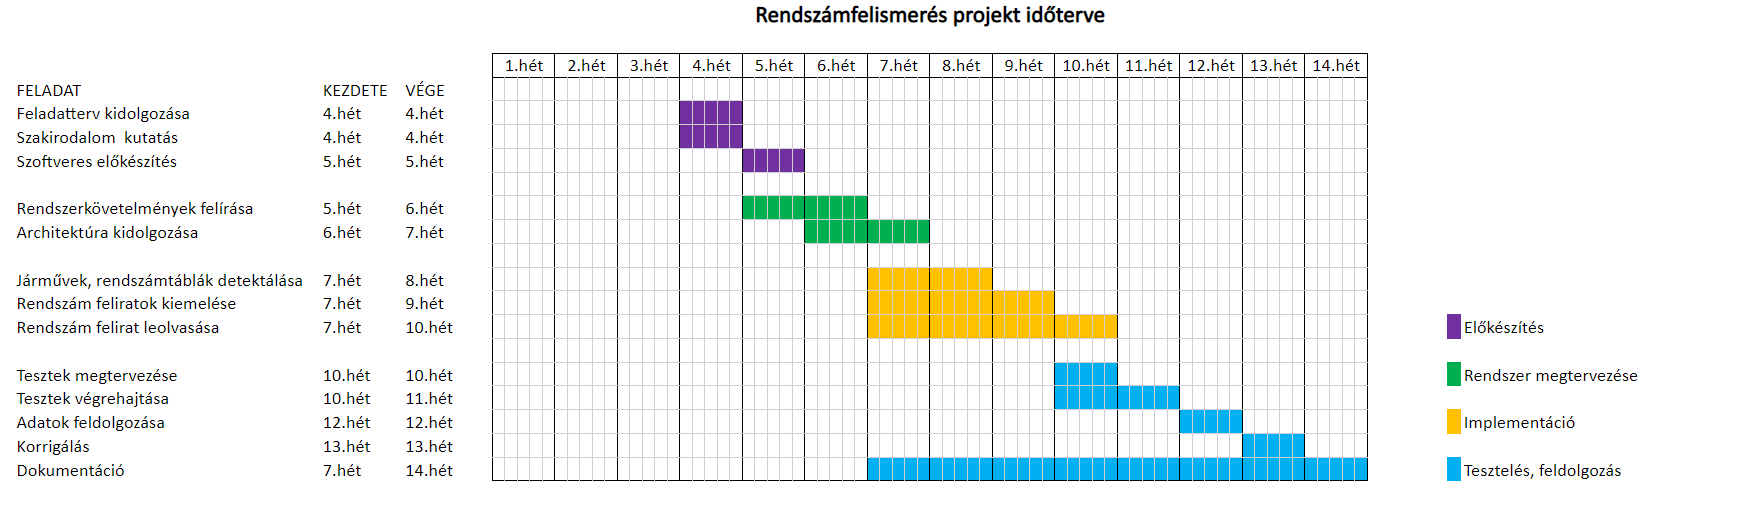
\includegraphics[width=1\columnwidth]{gannt.png}
        \caption{Időterv}
    \end{figure}
    \section{Fenntarthatóság}

        Már napjainkban is számos területen alkalmazunk rendszámfelismerést valamint ehhez kötött szolgáltatásokat, adatfeldolgozást. Különösen a közigazgatásban kerül felhasználásra, ugyanakkor a közeljövőben a környezetvédelemben is egy jelentős eszközzé válhat.
        \subsection{Közigazgatási folyamatok}
            A közigazgatás területén a rendszámfelismerés egy rendkívül fontos eszköz. Napjainkban számos szervezet alkalmazza ezen technológiát, gondoljunk csak az útdíjhasználat ellenőrzésére a világ számos országában (így többek között Magyarországon is). A technológia szolgálhat forgalom ellenőrzésére, rendőrségi eljárásokban autók nyomonkövetésére, kiszűrésére a forgalomból (ilyen a brit ANPR rendszer [HIVATKOZÁS 1], mely automatikusan szűri a biztrosítatlan illetve bűntényben résztvevő autókat egy központban), parkolókban a fizetés nyomonkövetésére illetve a járművek hatékonyabb be-és kiengedésében, továbbá behajtási jogosultság ellenőrzésére. Ezek mindegyike valamilyen módon segíti a közlekedés zökkenőmentességének fenntartását.

        \subsection{Környezetvédelem}
            A feljebb leírtak mellett a rendszámfelismerésnek mint technológiának a környezetvédelemben is egyre fontosabb szerepe van. Napjainkban számos nagyváros hoz létre emissziómentes zónákat, melyekben vagy behajtási tilalom, vagy pedig behajtási díjak (Londonban például ún. ,,congestion charge'' azaz dugódíj) van érvényben a járművek egy adott csoportjára. Ennek ellenőrzése és automatizálása rendszámfelismerő technológia nélkül kivitelezhetetlen, a technológia segítségével azonban egy rendkívül pontos és megbízható rendszer építhető ki, ezáltal is csükkentve a lokális légszennyezést városokban.

    \section{Eredmények dokumentálása}
        A rendszámfelismerő rendszerünket python programozási nyelven, az eggyüttműködés gördülékenységének érdekében github-on fogjuk fejleszteni. A dokumentáció \LaTeX-ben kerül megírásra, mely github-on is elérhető lesz.

    \section{Forrás}

        HIVATKOZÁS 1:
        https://www.police.uk/advice/advice-and-information/rs/road-safety/automatic-number-plate-recognition-anpr/

\end{document}